\section{Proposed architecture} \label{sec:proposed-arch}

By the end of the development phase, we created a system that fulfils all requirements described in \autoref{sec:requirements}.
The system mimics a typical DCS architecture by employing a simple master-slave configuration based on the EtherCAT network.

As explained in \autoref{subsec:local_remote}, using the local control topology (traditional topology), the master node will act as a motion controller, feeding the motor controller (the field device) with position/velocity references through the EtherCAT network.
This one, in turn, will perform the necessary algorithm calculations to achieve motor position/velocity control using the references provided by the master node and the feedback values it acquires from the motor's encoder.

When using the remote control topology, the master node will be responsible for all calculations in the system.
The field device will act as a simple I/O interface to the motor, generating the PWM waveform fed to the motor and acquiring and decoding the motor's encoder pulses.
The decoded position and velocity values are then sent to the master node as feedback variables and the PWM duty cycle percentage is received from it as an output variable.

Graphical representations of both these scenarios can be seen in \autoref{fig:local_control} and \autoref{fig:remote_control}, respectively. \footnote{NOTE: These are placeholder images, I will replace them with better images or graphs designed by me}


\begin{figure}[t]
	\centering
	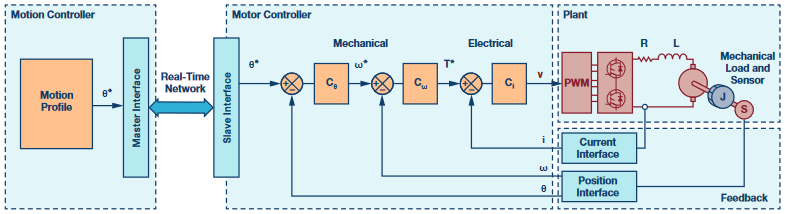
\includegraphics[width=1\textwidth]{local_control.png}
	\caption{Graphical representation of the local control scheme}
	\label{fig:local_control}
\end{figure}

\begin{figure}[t]
	\centering
	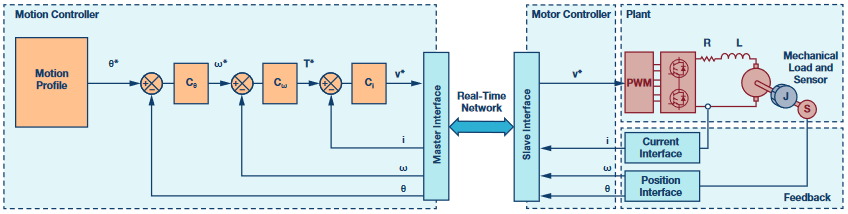
\includegraphics[width=1\textwidth]{remote_control.png}
	\caption{Graphical representation of the remote control scheme}
	\label{fig:remote_control}
\end{figure}


\subsection{Hardware} \label{sec:proposed-hardware}

While keeping a careful consideration of characteristics between options and maintaining the requirements in focus, hardware parts were chosen to build each section of the demonstrator.

\subsubsection{Master node}

Taking into account the two operation modes the demonstrator should have, we extrapolated that the master node must be able to perform numeric calculations and serve as an EtherCAT master device.
As the EtherCAT master implementation can be done using a generic Ethernet MAC interface card (refer to \ref{subsubsec:master_devices} for an explanation), everything the master node requires in term of hardware is a computational platform (computer, microcontroller, etc.) with access to a generic Ethernet MAC interface card.

As of today, most education facilities provide students with access to desktop computers.
For many years now, motherboard vendors have integrated Ethernet MAC interface cards into the motherboards themselves, as it has become the \emph{de facto} standard for Internet connectivity in desktop computers.

As such, we decided to implement the master device in a desktop computer in order to minimize costs and leverage the computational power modern computer systems possess.

\subsubsection{Slave node} \label{subsubsec:slave_hdw}

On the other hand, the slave node's hardware was harder to choose.
In order to implement the desired EtherCAT slave (see \ref{subsubsec:slave_devices}), one must be aware when choosing a computational platform to check the availability of a fitting ESC board and, simultaneously, the support for motor and encoder interfaces.

After some research, two options presented themselves as possible platforms for the slave device: an Arduino UNO or a Raspberry Pi.
ESC boards exist for both these platforms, as well as good support in terms of "shield boards" for motor interfaces.
In the end, we decided to go with a solution based on a Raspberry Pi, as it provides a more robust and versatile computing platform, especially considering the local control configuration, where position/velocity control algorithms will need to be executed on this platform.

The ESC board chosen for the Raspberry Pi was the Hilscher's \emph{netHAT 52-RTE} (see \url{www.netiot.com/interface/nethat}).
This board supports communication with three real-time Ethernet protocols (PROFINET, EtherNet/IP or EtherCAT), chosen with a simple firmware loading procedure.
It complies with the Hardware Attached on Top (HAT) specification for the Raspberry Pi (see \url{www.github.com/raspberrypi/hats}) and uses the \emph{SPI0} interface to communicate with it.
The board also includes the respective Electronic Data Sheet (EDS) files to be imported by the EtherCAT master, used to identify the characteristics and functionality of slaves implemented using this setup.

% Motor choice

With the intention to relieve the Raspberry Pi from having to generate the PWM signal to drive the motor, we included the DFRobot's DFR0592 board onto the design.
This board also complies with the HAT specification and communicates with the Raspberry Pi via the Inter-Integrated Circuit (I\textsuperscript{2}C or I2C) interface.
It provides interface with two DC motors and two incremental encoders, all managed by an STMicroelectronics's STM32 chip.
The motor interface also includes the necessary DC-motor driver chip, allowing direct connection of the motor's terminals and power supply to the board itself.

Initially we planed on using this board's incremental encoder interface to also relieve the Raspberry Pi from such task but, as our preliminary tests concluded, it only exports the Revolutions Per Minute (RPM) value extrapolated from the encoder's pulse count and not the pulse count itself.
Furthermore, the RPM value is only updated once every 100ms, which is to large of a period for motion control.

\begin{figure}[htp]
	\centering
	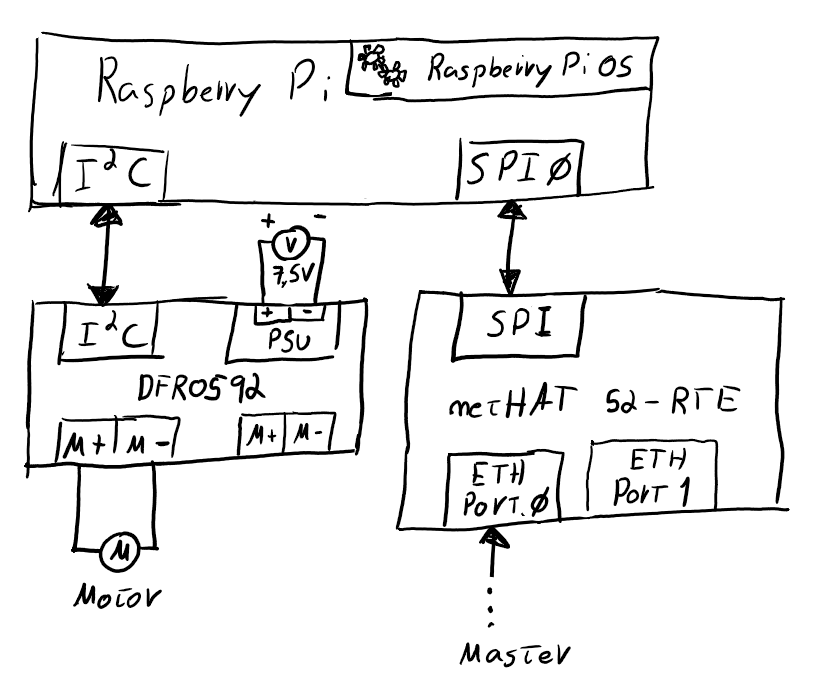
\includegraphics[width=1\textwidth]{slave_architecture.png}
	\caption{Graphical representation of the remote control scheme}
	\label{fig:slave_architecture}
\end{figure}\footnote{placeholder image}


\subsection{Software} \label{sec:proposed-software}

As can be expected, recent digital computing platforms require software to perform the necessary tasks.
As such, both the master node (computer) and the slave device (Raspberry Pi) will each require an Operating System (OS) to manage the execution of tasks.
The Raspberry Pi has a dedicated Linux OS called \emph{Raspberry Pi OS}, which is a fork from Debian (see \url{https://www.raspberrypi.org/software/}.
We will be using the Lite version of this OS for the Raspberry Pi as it is the easiest to setup and the most tested and stable OS for this platform.
Regarding the master node computer we will be using Microsoft's Windows 10 as the chosen OS, not only because most computers come pre-installed with it, but also because it is one of the few supported OSes by the CODESYS development application \cite{ide:codesys}, presented below.

\subsubsection{Master node software}

In order for us to create a control application on a generic computer, an appropriate software platform must be chosen.
Because we are working with industrial technology, a proper industrial control and automation software should be used.

CODESYS is a generic platform to develop industrial control and automation applications based on the IEC 61131-3 standard.
It includes support for hardware from multiple vendors as well as the ability to create a Software PLC (SoftPLC) from any generic computer hardware.
This platform makes the software editor available to use for free and allows control applications to run for two hours in demonstration/testing mode, uninterrupted.
This is a great option for development and testing purposes as only the final product with uninterrupted execution requirements for unknown periods of time will require a license to be purchased.
Additionally, CODESYS natively supports the most common industrial communication networks, including EtherCAT, meaning one can develop a device with communication capabilities with one or more of these networks.

With all this, we will use the CODESYS platform to create a SoftPLC to act as an EtherCAT master device for or demonstrator.
As we are looking forward to develop a proof-of-concept system, we don't require application runtimes larger than two hours.

Because we want to involve the end-user into the process of setting-up and running the experiments by themselves, we decided to leave the implementation of the master node's software to be dealt with by the end-user.
By doing such, we will also be indirectly expanding the set of conceptual experiments the demonstrator can handle by allowing anyone to implement their own ideas, as the slave device will always work the same way.

\subsubsection{Slave node software}

After having chosen the Hilscher's ESC HAT for the Raspberry Pi (see \ref{subsubsec:slave_hdw}), which will be running a Linux distribution, and decided to use the CODESYS platform for the master, we initially planned to also use CODESYS to program the slave device.
Although its editor is only designed to work under Windows, the SoftPLC runtime can run under Linux, with a version specifically targeting the Raspberry Pi platform.
Unfortunately, CODESYS doesn't support developing programs for EtherCAT slave devices, specifically, as these are usually programmed by manufacturers themselves and not by a system integrator or end-user.

Additionally, Hilscher only provides a library and accompanying API definitions for the C programming language, meaning at least the software module that needs to interact directly with the ESC will need to be programmed in C language.
As this is the most widely used programming language in the Linux universe, if during development we conclude we require some library to provide us with some advanced functionality, the probability of existing one for the C language is much higher than with less widespread languages.
As such, this is going to be our preferred programming language for implementing the EtherCAT's slave software running on the Raspberry Pi.



